
\begin{figure}[h!]
    \centering
    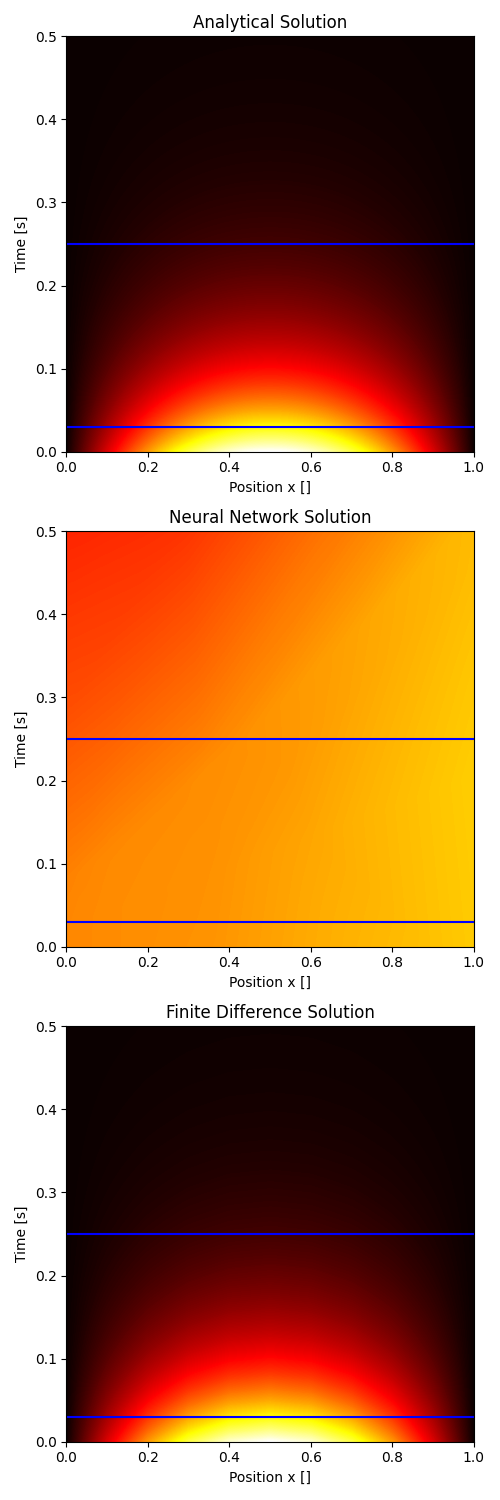
\includegraphics[width=1.0\linewidth]{project_3/plots/heat_map_comparison.png}
    \caption{The analytical solution to the heat equation, and the results from the finite difference method and the neural network model. A common color bar is displayed as all three plots have the same range of values [0,1]. The blue lines indicate the times $t = 0.03 s$ and $t = 0.25 s$.}
    \label{fig:heatmaps}
\end{figure}

The results from the finite difference method and the NN are presented in Fig. \ref{fig:heatmaps}.
The outputs from the models have been interpolated for the plots. \gaute{more}
There is no noticeable difference by eye between any of the three.  
This is well reflected in the very low MSE-value for both methods. 
Compared to the analytical solution, the output of the neural network model has an MSE of $ 6.71 \times 10^{-6}$ while the finite difference method yields an MSE of $2.52 \times 10^{-7}$. 
Since the two methods utilize different discretizations of the $(x,t)$ grid, the analytical solution is evaluated only at the respective grid points of each method. 
Consequently, the MSE calculation for the neural network involves a greater number of points than that of the finite difference method.
\mia{impact?}


\begin{figure}[h!]
    \centering
    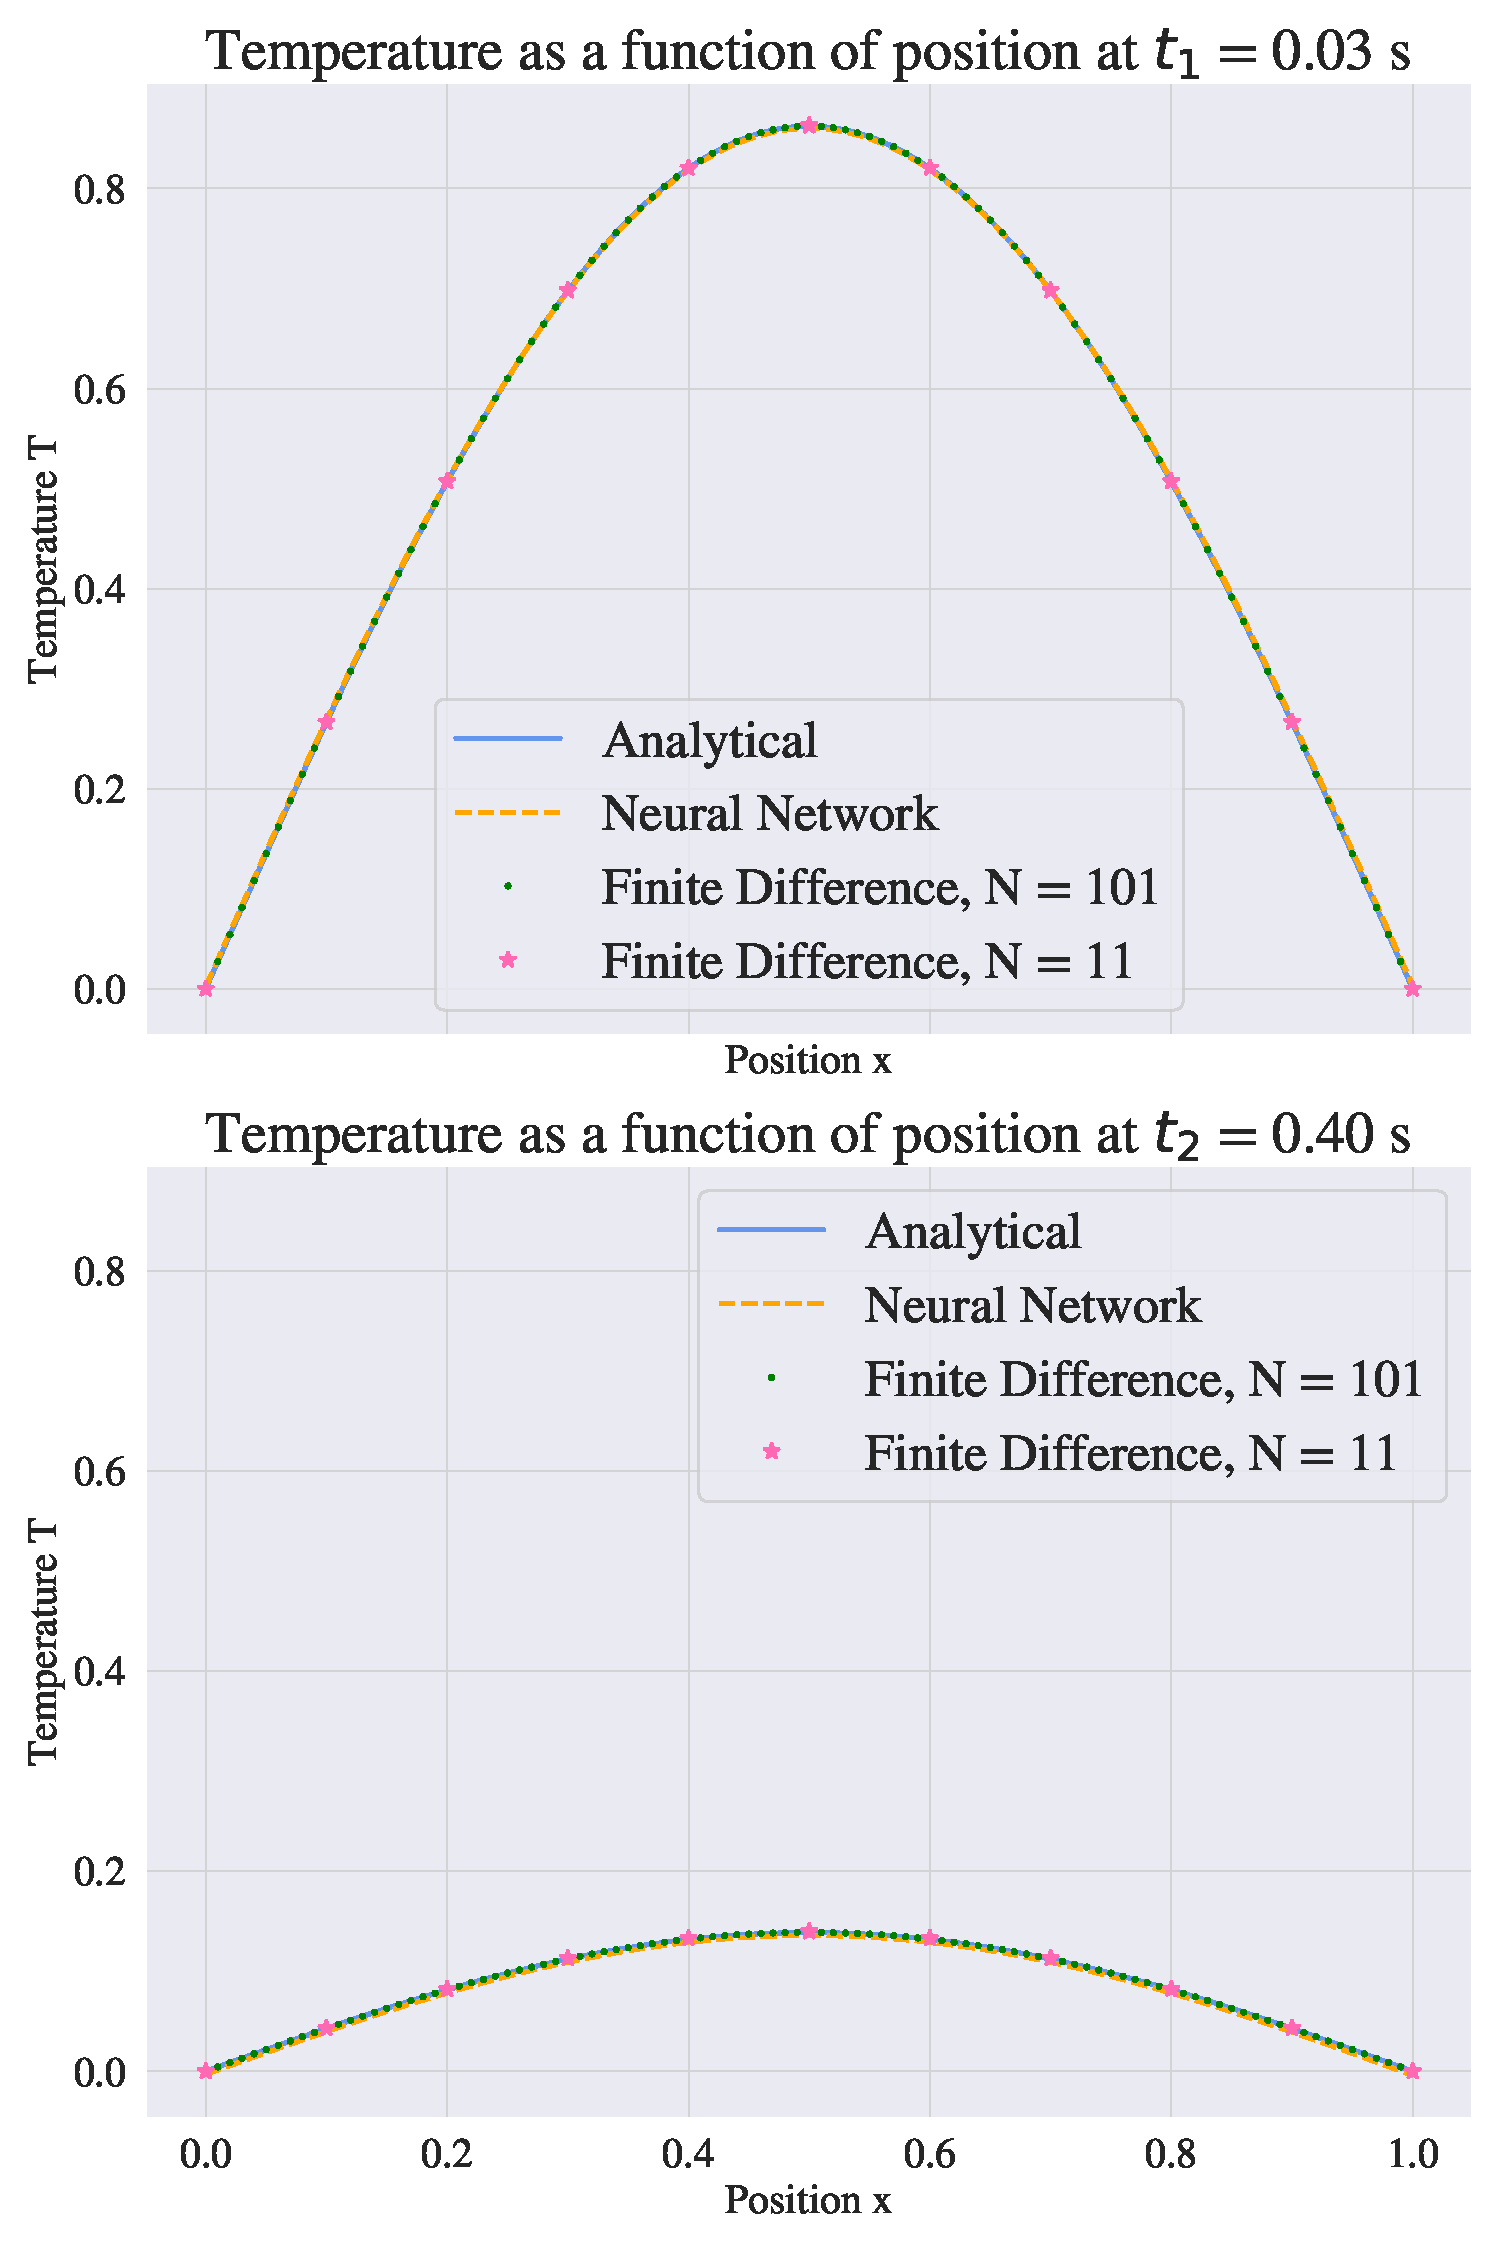
\includegraphics[width=1.0\linewidth]{project_3/plots/time_slices_comparison.pdf}
    \caption{The temperature for specific times for the analytical solution, as well as the output from the finite difference method and the neural network predictions. The discretization along the x-axis is different for each method. The analytical one is plotted with 1000 points, the finite difference method with 10 points, and the neural network predictions with 100. }
    \label{fig:timeslices}
\end{figure}


We \textit{"slice"} the heatmaps in Fig. \ref{fig:heatmaps} at two specific times, $t = 0.03 s$ and $t = 0.25 s$. 
This is illustrated as blue lines in Fig. \ref{fig:heatmaps}.
The resulting temperature values across the x-range are plotted for all three cases in Fig. \ref{fig:timeslices}.
\mia{something about the choice of the two times, ref the assignment}
This serves as an additional verification of the previously presented results. 
The finite difference method seems to match the analytical solution perfectly \mia{strong word?}.
The NN however, is slightly undershooting. 
The effect of this is more prominent for the later time stamp $t = 0.25 s$. 
These results reflect well the lower MSE for the finite difference method compared to the NN. 
\mia{The reason for this might be: }


\mia{Additionally, the finite difference method with 100 points along the x-axis is plotted to illustrate what???}

\mia{why is N = 10 and N = 100 equally good for fd?}


The results from the in-depth investigation of the impact of the hyperparameters \textit{number of hidden layers}, the \textit{size of the hidden layers}, and the \textit{activation functions} are presented in Figs. \ref{fig:boxplots_activations}, \ref{fig:boxplots_size_of_layers} and \ref{fig:boxplots_number_of_hidden_layers} respectively. 
From the three-dimensional grid search, the best values were found to be three hidden layers with size 50 and tanh as the activation function.


\begin{figure}[h!]
    \centering
    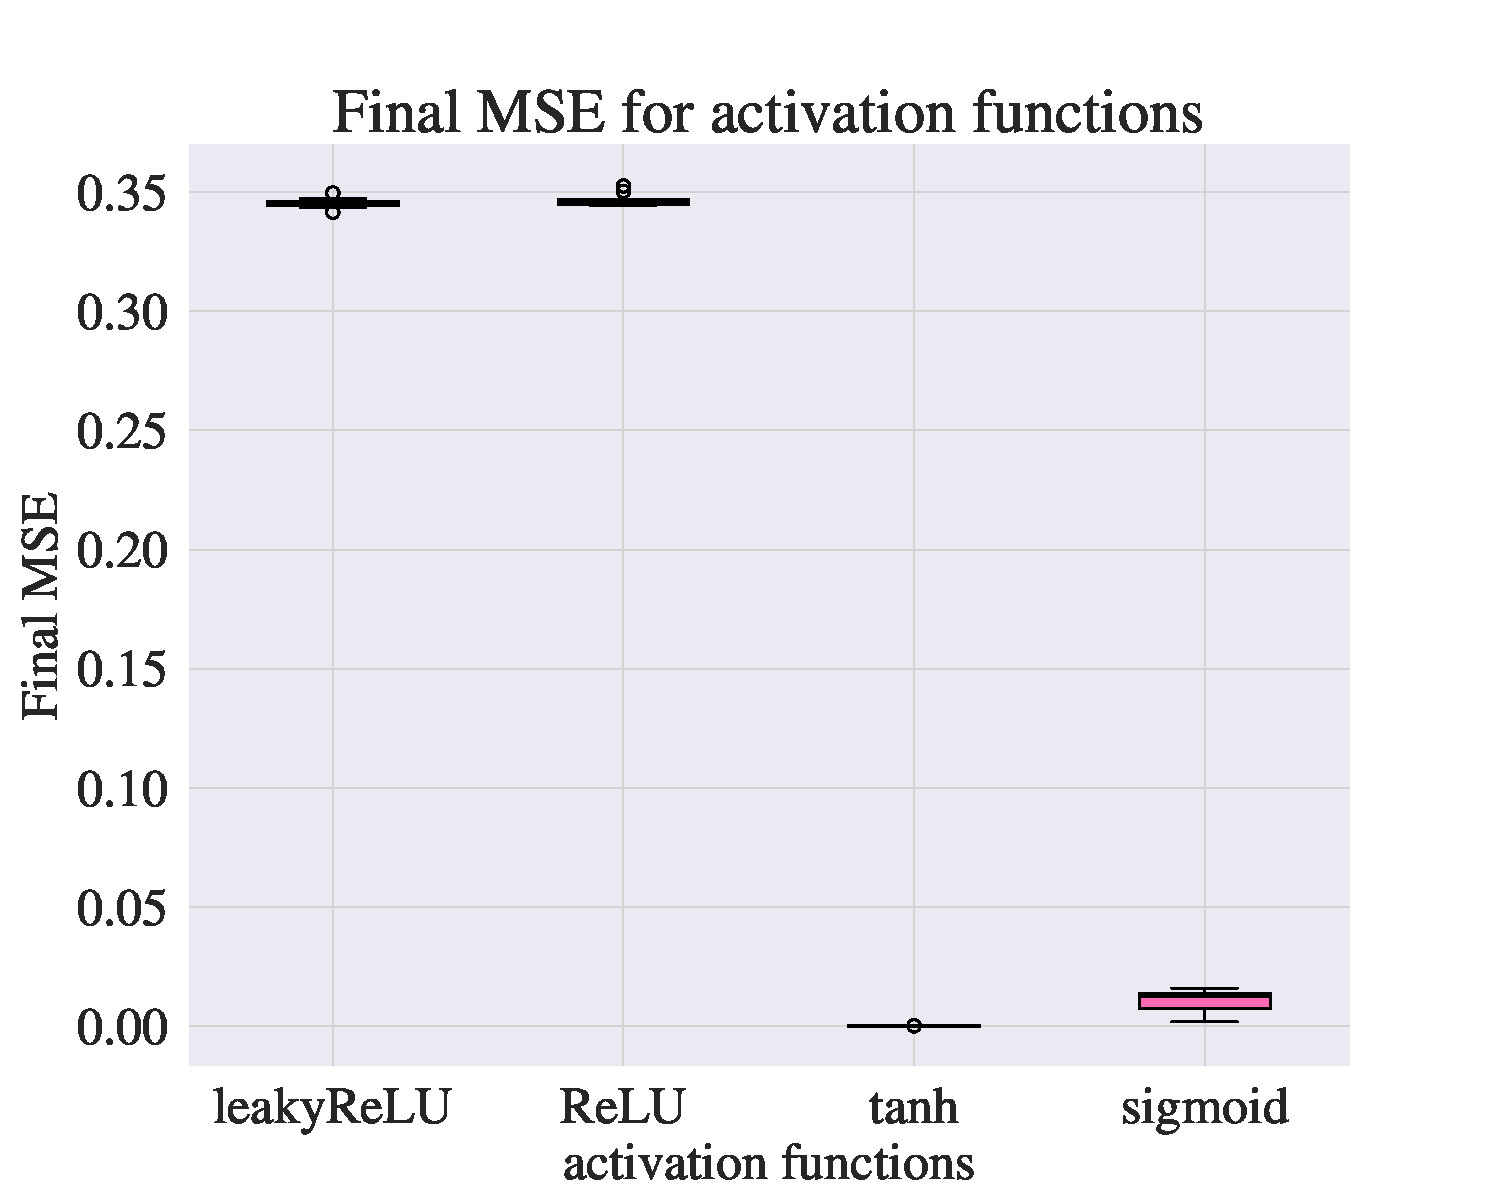
\includegraphics[width=1.0\linewidth]{project_3/plots/activation_search.pdf}
    \caption{Boxplots showcasing the final MSE value compared to the analytical solution for different activation functions. Each model is run 10 times.}
    \label{fig:boxplots_activations}
\end{figure}

As activation functions, sigmoid and tanh outperform ReLU and leakyReLU. 
\mia{why}

\begin{figure}[h!]
    \centering
    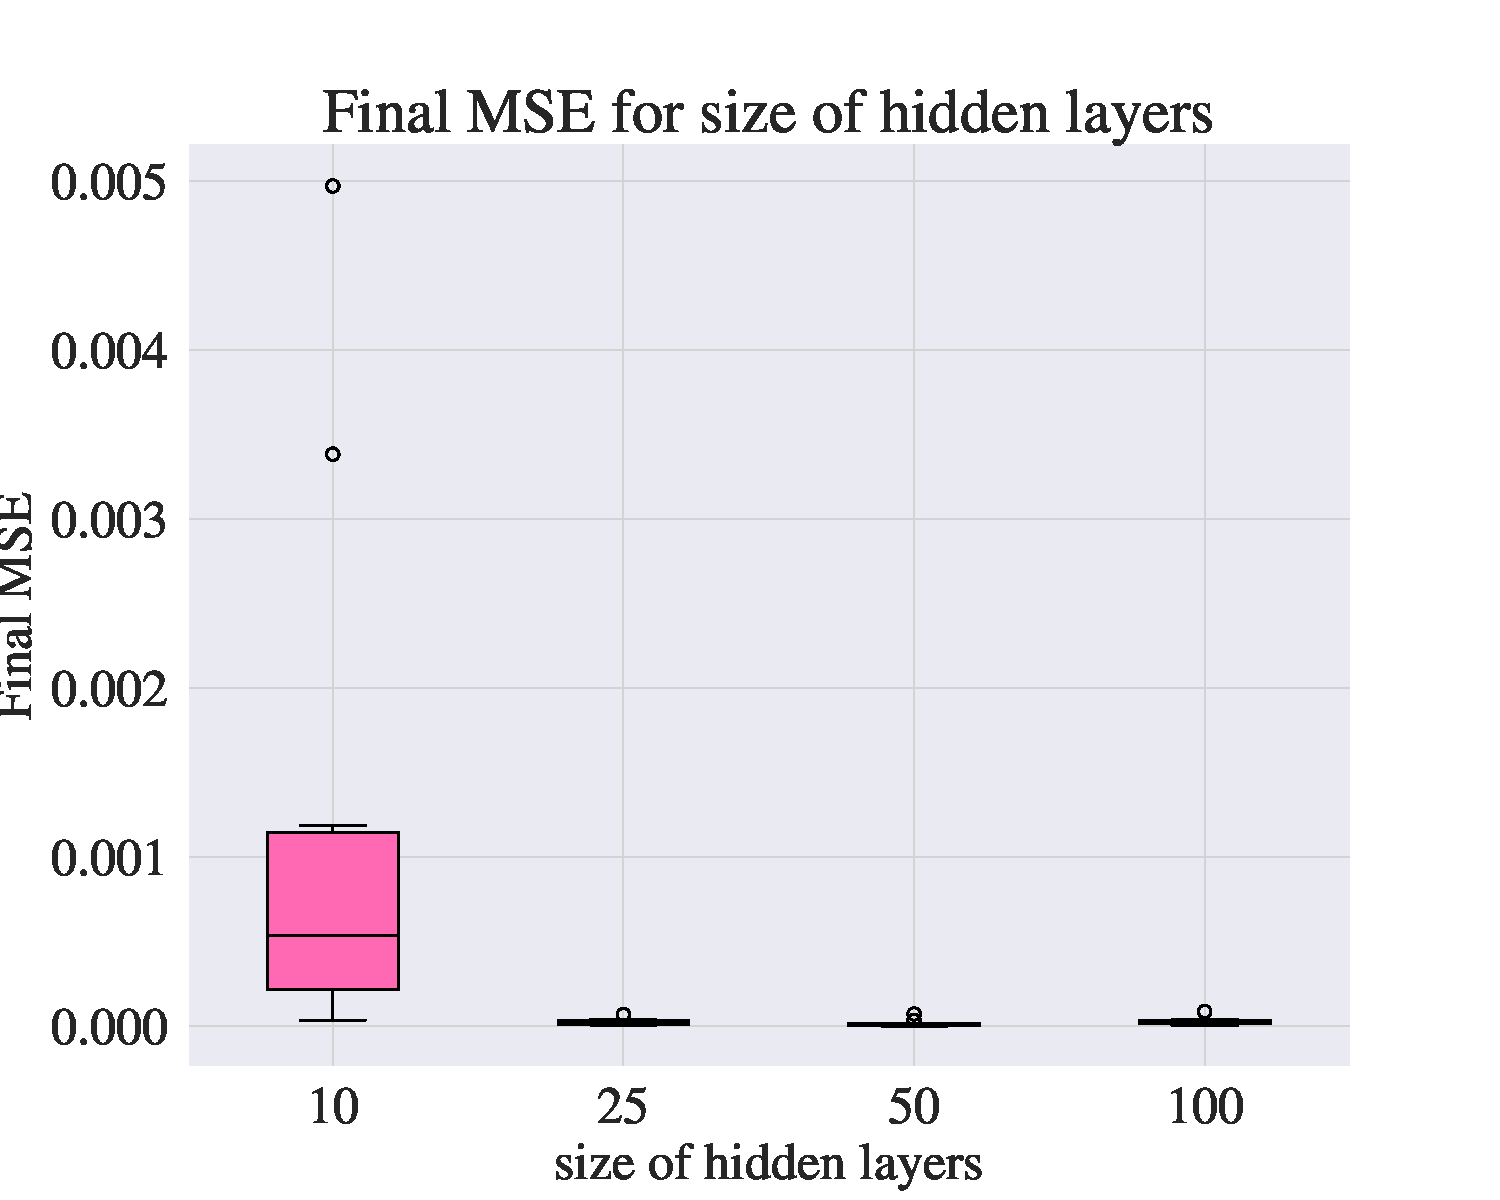
\includegraphics[width=1.0\linewidth]{project_3/plots/value_layers_search.pdf}
    \caption{Boxplots showcasing the final MSE value compared to the analytical solution for different sizes for the hidden layers. Each model is run 10 times. \mia{this is wrong plot for now}}
    \label{fig:boxplots_size_of_layers}
\end{figure}

\mia{fill inn}

\begin{figure}[h!]
    \centering
    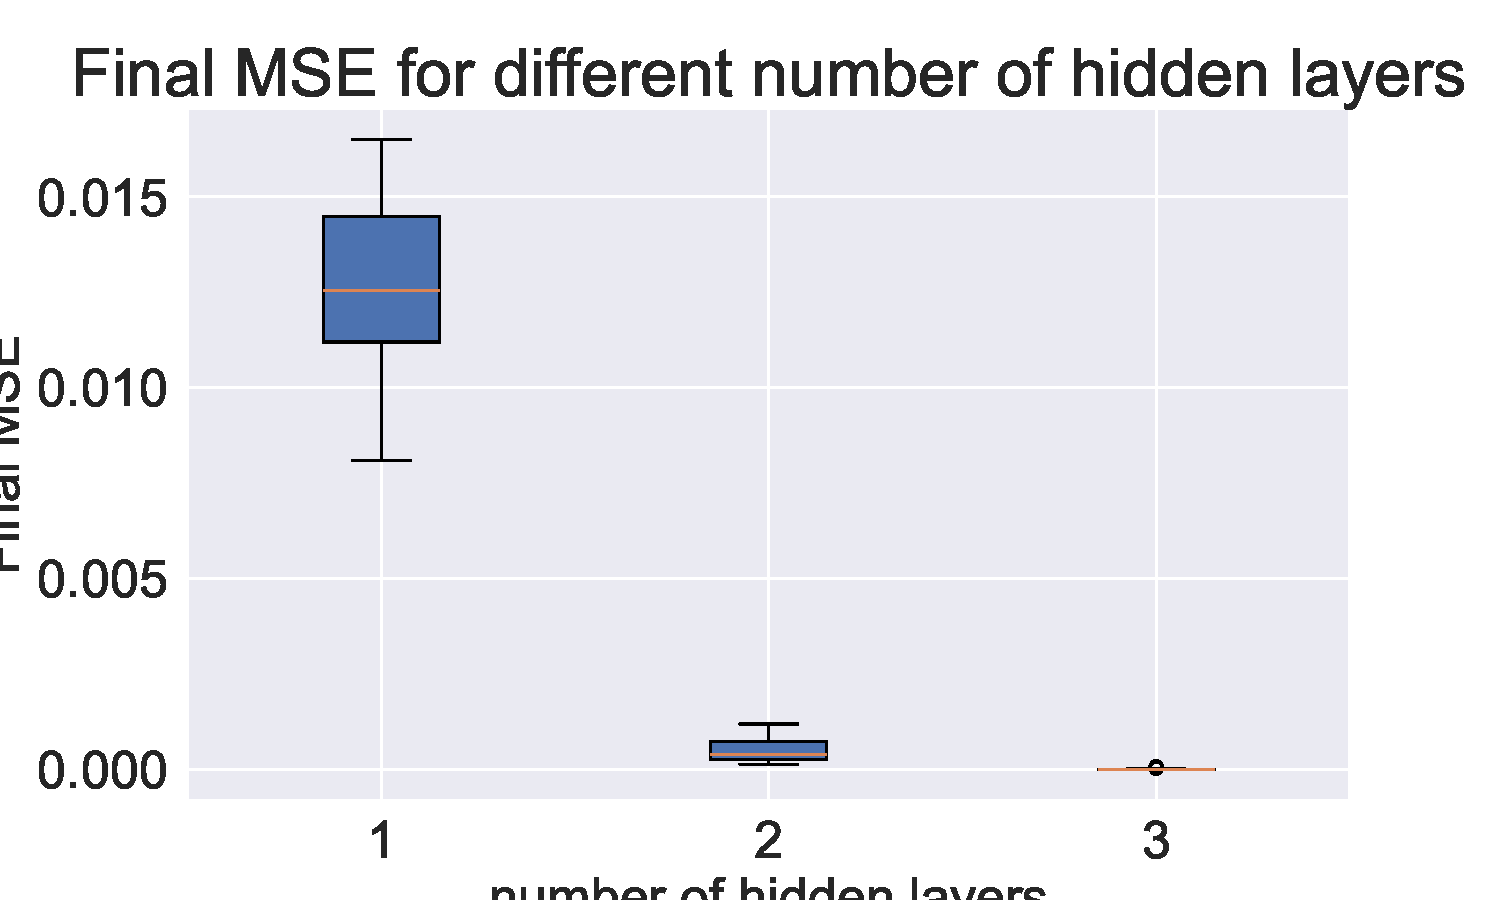
\includegraphics[width=1.0\linewidth]{project_3/plots/n_layers_search.pdf}
    \caption{Boxplots showcasing the final MSE value compared to the analytical solution for different numbers of hidden layers. Each model is run 10 times.}
    \label{fig:boxplots_number_of_hidden_layers}
\end{figure}
